% !TEX program=lualatex
\RequirePackage{luatex85}
\documentclass[11pt,tikz]{standalone}
\usepackage[utf8]{inputenc}
\usepackage[T1]{fontenc}
\usepackage{textcomp}
\usepackage[scaled]{helvet}
\usepackage{tikz}
\usetikzlibrary{shapes,arrows,positioning}
\renewcommand{\familydefault}{\sfdefault}

\tikzstyle{line}=[draw, ->, very thick]
\tikzstyle{sq}=[rectangle,draw=black!60,fill=black!5,very thick,on grid]

\begin{document}
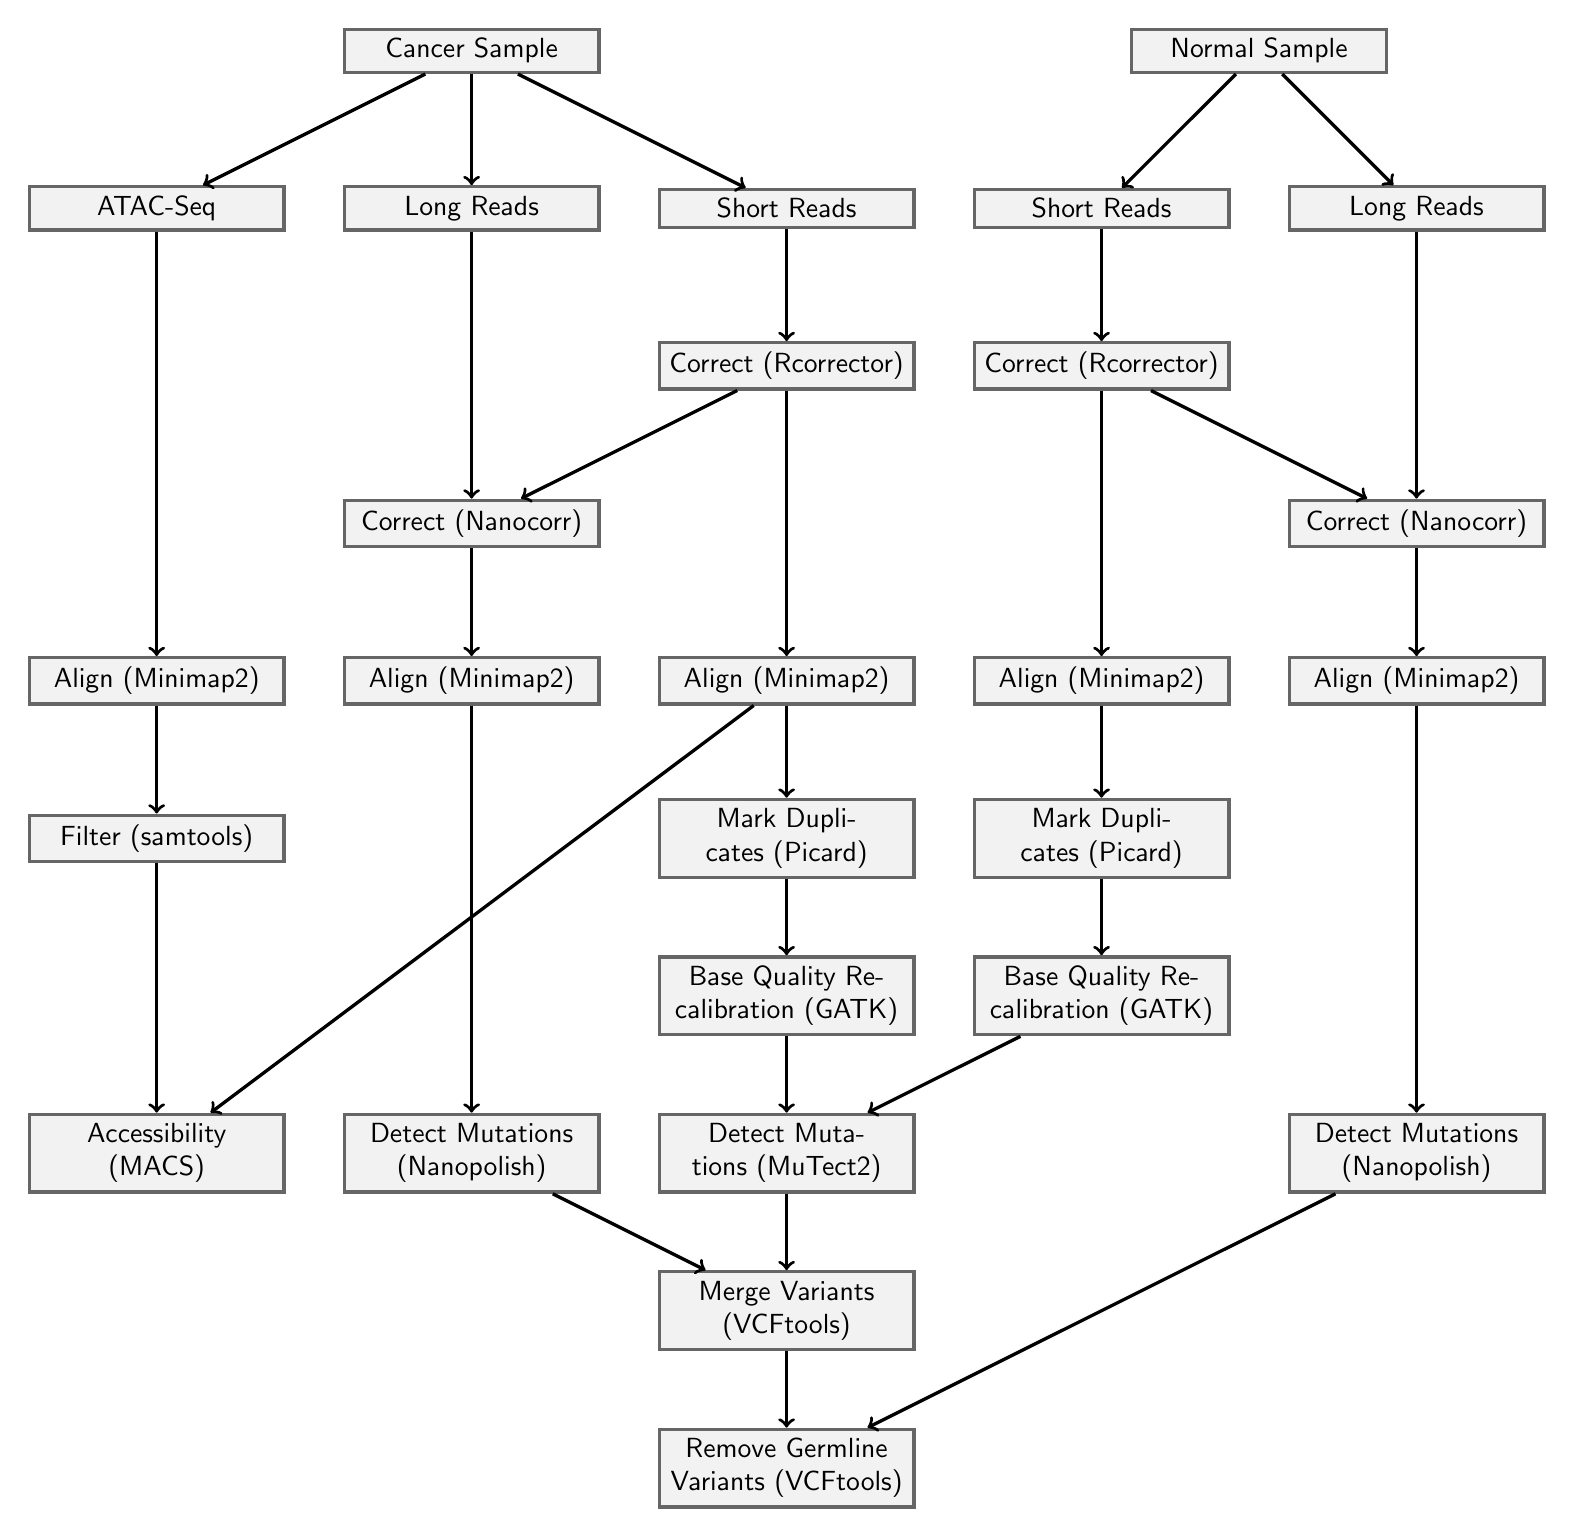
\begin{tikzpicture}[node distance=20mm, text width = 30mm, align = center,auto]

% \draw[step=1cm,gray,very thin] (-10,-30) grid (20,10);

%cancer
\node[sq] (cancer) {Cancer Sample};

%atac
\node[sq, below left = 2 and 4 of cancer] (atac) {ATAC-Seq};
\node[sq, below = 6 of atac] (ataca) {Align (Minimap2)};
\node[sq, below = of ataca] (atacf) {Filter (samtools)};
\node[sq, below = 4 of atacf] (macs) {Accessibility (MACS)};

%long reads
\node[sq, below = 2 of cancer] (lr) {Long Reads};
\node[sq, below = 4 of lr] (lrc) {Correct (Nanocorr)};
\node[sq, below = of lrc] (lra) {Align (Minimap2)};
\node[sq, below = 6 of lra] (lrd) {Detect Mutations (Nanopolish)};

%short reads
\node[sq, below right = 2 and 4 of cancer] (sr) {Short Reads};
\node[sq, below = of sr] (src) {Correct (Rcorrector)};
\node[sq, below = 4 of src] (sra) {Align (Minimap2)};

\node[sq, below = of sra] (srmd) {Mark Duplicates (Picard)};
\node[sq, below = of srmd] (srb) {Base Quality Recalibration (GATK)};
\node[sq, below = of srb] (srd) {Detect Mutations (MuTect2)};

%combo
\node[sq, below = of srd] (srv) {Merge Variants (VCFtools)};
\node[sq, below = of srv] (srg) {Remove Germline Variants (VCFtools)};

%normal
\node[sq, right= 10 of cancer] (normal) {Normal Sample};

%short
\node[sq, below left = 2 and 2 of normal] (nsr) {Short Reads};
\node[sq, below = of nsr] (nsrc) {Correct (Rcorrector)};
\node[sq, below = 4 of nsrc] (nsra) {Align (Minimap2)};
\node[sq, below = of nsra] (nsrmd) {Mark Duplicates (Picard)};
\node[sq, below = of nsrmd] (nsrb) {Base Quality Recalibration (GATK)};

%long
\node[sq, below right = 2 and 2 of normal](nlr) {Long Reads};
\node[sq, below = 4 of nlr] (nlrc) {Correct (Nanocorr)};
\node[sq, below = of nlrc] (nlra) {Align (Minimap2)};
\node[sq, below = 6 of nlra] (nlrd) {Detect Mutations (Nanopolish)};

%arrows
%atac
\draw[line] (cancer) -- (atac);
\draw[line] (atac) -- (ataca);
\draw[line] (ataca) -- (atacf);
\draw[line] (atacf) -- (macs);

%lr
\draw[line] (cancer) -- (lr);
\draw[line] (lr) -- (lrc);
\draw[line] (lrc) -- (lra);
\draw[line] (lra) -- (lrd);

%sr
\draw[line] (cancer) -- (sr);
\draw[line] (sr) -- (src);
\draw[line] (src) -- (sra);
\draw[line] (sra) -- (srmd);
\draw[line] (srmd) -- (srb);
\draw[line] (srb) -- (srd);
\draw[line] (srd) -- (srv);
\draw[line] (srv) -- (srg);

%normal - short
\draw[line] (normal) -- (nsr);
\draw[line] (nsr) -- (nsrc);
\draw[line] (nsrc) -- (nsra);
\draw[line] (nsra) -- (nsrmd);
\draw[line] (nsrmd) -- (nsrb);
\draw[line] (nsrb) -- (srd);

%normal - long
\draw[line] (normal) -- (nlr);
\draw[line] (nlr) -- (nlrc);
\draw[line] (nlrc) -- (nlra);
\draw[line] (nlra) -- (nlrd);
\draw[line] (nlrd) -- (srg);

%normal combo
\draw[line] (nsrc) -- (nlrc);
\draw[line] (lrd) -- (srv);

%cancer combo
\draw[line] (src) -- (lrc);
\draw[line] (sra) -- (macs);

\end{tikzpicture}
\end{document}

